\section{Protocol}

\subsection{Frozen Data Roles}

GlaS official train remains divided into a 55-image utility pool and a 30-image strict-validation query pool. The 55 images are further split into 40 calibration images and 15 internal method-selection images. GlaS testA and testB remain locked and unused. The statistical unit is the query image; three references per query are repeated measurements and are not independent samples.

\subsection{Frozen Evidence and Region Bank}

The matcher is frozen DINOv2-L with the pre-registered local-peaks candidate redesign that passed GlaS Gate C. No new matcher, feature extractor, threshold grid, or region action is added after strict validation. Query-level evidence is defined by pre-registered aggregation over the three references. Region actions are bounded by the bank in Table~\ref{tab:region_actions}.

\begin{table*}[t]
\centering
\small
\caption{Pre-registered Phase 3 region action bank. Privileged upper bounds are separated from automatic actions.}
\label{tab:region_actions}
\begin{tabular}{llllll}
\hline
ID & Action & Type & Calls & Role & Phase 3 note \\
\hline
R00 & Direct matching mask & mask & 0 & automatic & raw proposal baseline \\
R01 & Full-image box & box & 1 & control & trivial control \\
R02 & Size-matched random box & box & 1 & control & matched random control \\
R03 & Automatic union box & box & 1 & automatic & tight union of proposals \\
R04 & Largest-component box & box & 1 & automatic & largest proposal component \\
R05 & Top-3 component boxes & box & <=3 & automatic & largest three components \\
R06 & Hard mask prompt & mask & 1 & automatic & blocked by R1 \\
R07 & Soft-logit mask prompt & mask & 1 & automatic & blocked by R1 \\
R08 & Box + soft mask & hybrid & 1 & automatic & blocked by R1 \\
R09 & Top-point baseline & point & 1 & automatic & not grouped P3 reopening \\
U01-U03 & GT region upper bounds & privileged & 1-3 & upper bound & not automatic \\
\hline
\end{tabular}
\end{table*}

\begin{table*}[t]
\centering
\small
\caption{Global region configurations selected before strict validation. Selection used only the 40/15 internal protocol.}
\label{tab:selected_configs}
\begin{tabular}{lllllll}
\hline
Family & Aggregation & q & min area & closing & top k & positive limit \\
\hline
R00 direct matching mask & mean & 0.7 & 0.001 & 5 & 1 & 20 \\
R03 automatic union box & mean & 0.7 & 0.001 & 5 & 1 & 20 \\
R04 automatic largest component box & mean & 0.7 & 0.001 & 5 & 1 & 20 \\
R05 automatic top3 component boxes & mean & 0.7 & 0.001 & 5 & 3 & 20 \\
\hline
\end{tabular}
\end{table*}


\subsection{Gate R1}

Gate R1 evaluates proposal quality before any new SAM region inference. A box route must improve mean box IoU over size-matched random boxes by at least 0.10, win on at least 70 percent of queries, reach foreground recall at least 0.70, and keep empty proposals at or below 0.10. A mask route must reach mean raw-mask Dice at least 0.30, improve over matched controls by at least 0.15, reach foreground recall at least 0.60, and keep empty proposals at or below 0.10.

Failure of all automatic families triggers \texttt{STOP\_GLAS\_REGION\_PROPOSAL\_FAILURE}. Under that state, R2 SAM region inference, R3 oracle analysis, router training, and formal test access are prohibited.

\begin{figure*}[t]
\centering
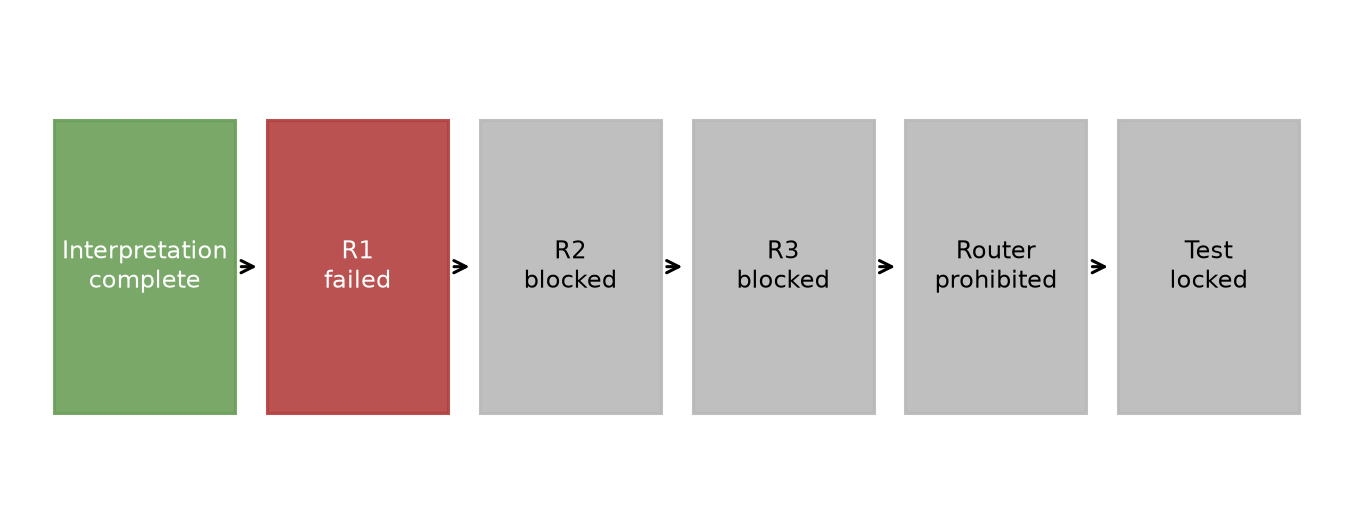
\includegraphics[width=.95\textwidth]{figures/phase3_gate_state_flow.png}
\caption{Phase 3 state flow. R1 proposal quality fails, so downstream SAM refinement, oracle analysis, router training, and formal tests are blocked by protocol.}
\label{fig:gate_flow}
\end{figure*}
